% Real CFG fragment from the ELF evaluation.
% Addresses, function names, and labels are taken from out.dot produced
% by ParseRE on May 21, 2026. All 12 blocks shown received the
% section_header label.
\documentclass[tikz,border=10pt]{standalone}
\usepackage{tikz}
\usepackage{xcolor}
\usetikzlibrary{positioning,arrows.meta,fit,backgrounds}

\definecolor{seccol}{HTML}{6C8B3F}
\definecolor{harncol}{HTML}{4A7AB7}
\definecolor{libcol}{HTML}{D97757}
\definecolor{bgcol}{HTML}{F8F6EF}

\begin{document}
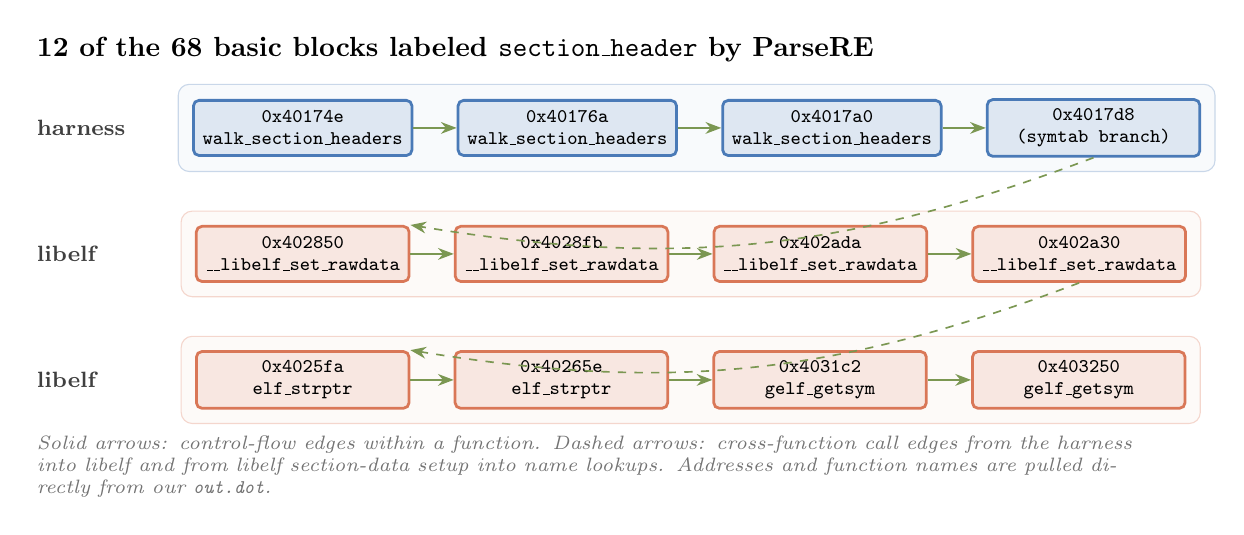
\begin{tikzpicture}[
  font=\sffamily\footnotesize,
  node distance=0.45cm and 0.55cm,
  bb/.style={
    draw=#1, fill=#1!18, line width=1.0pt,
    rounded corners=2pt,
    minimum height=0.7cm, minimum width=2.7cm, align=center,
    font=\scriptsize\ttfamily,
  },
  arrow/.style={-{Stealth[length=2mm]}, line width=0.6pt, draw=seccol!90},
  grouplabel/.style={font=\bfseries\footnotesize, anchor=west, text=black!75},
  caption/.style={font=\scriptsize\itshape, text=black!55},
]

% =================== GROUP 1: harness ===================
\node[bb=harncol] (h1) at (0, 4.6) {0x40174e\\walk\_section\_headers};
\node[bb=harncol, right=of h1] (h2) {0x40176a\\walk\_section\_headers};
\node[bb=harncol, right=of h2] (h3) {0x4017a0\\walk\_section\_headers};
\node[bb=harncol, right=of h3] (h4) {0x4017d8\\(symtab branch)};

\draw[arrow] (h1) -- (h2);
\draw[arrow] (h2) -- (h3);
\draw[arrow] (h3) -- (h4);

% =================== GROUP 2: libelf section setup ===================
\node[bb=libcol] (l1) at (0, 3.0) {0x402850\\\_\_libelf\_set\_rawdata};
\node[bb=libcol, right=of l1] (l2) {0x4028fb\\\_\_libelf\_set\_rawdata};
\node[bb=libcol, right=of l2] (l3) {0x402ada\\\_\_libelf\_set\_rawdata};
\node[bb=libcol, right=of l3] (l4) {0x402a30\\\_\_libelf\_set\_rawdata};

\draw[arrow] (l1) -- (l2);
\draw[arrow] (l2) -- (l3);
\draw[arrow] (l3) -- (l4);

% =================== GROUP 3: libelf lookups ===================
\node[bb=libcol] (s1) at (0, 1.4) {0x4025fa\\elf\_strptr};
\node[bb=libcol, right=of s1] (s2) {0x40265e\\elf\_strptr};
\node[bb=libcol, right=of s2] (s3) {0x4031c2\\gelf\_getsym};
\node[bb=libcol, right=of s3] (s4) {0x403250\\gelf\_getsym};

\draw[arrow] (s1) -- (s2);
\draw[arrow] (s2) -- (s3);
\draw[arrow] (s3) -- (s4);

% Cross-group arrows showing real edges from out.dot
\draw[arrow, dashed] (h4.south) to[bend left=15] (l1.north east);
\draw[arrow, dashed] (l4.south) to[bend left=15] (s1.north east);

% Group labels
\node[grouplabel] at (-3.5, 4.6) {harness};
\node[grouplabel] at (-3.5, 3.0) {libelf};
\node[grouplabel] at (-3.5, 1.4) {libelf};

% Background boxes
\begin{scope}[on background layer]
  \node[fit=(h1)(h4), draw=harncol!30, fill=harncol!4, rounded corners=4pt, inner sep=5pt] {};
  \node[fit=(l1)(l4), draw=libcol!30, fill=libcol!4, rounded corners=4pt, inner sep=5pt] {};
  \node[fit=(s1)(s4), draw=libcol!30, fill=libcol!4, rounded corners=4pt, inner sep=5pt] {};
\end{scope}

% Title and caption
\node[font=\bfseries, anchor=west] at (-3.5, 5.6) {12 of the 68 basic blocks labeled \texttt{section\_header} by ParseRE};
\node[caption, anchor=west, text width=14cm, align=left] at (-3.5, 0.3)
  {Solid arrows: control-flow edges within a function. Dashed arrows: cross-function call edges from the harness into libelf and from libelf section-data setup into name lookups. Addresses and function names are pulled directly from our \texttt{out.dot}.};

\end{tikzpicture}
\end{document}
